\hoofdstuk{Main research}
Work in progress.

This chapter will define the main research process. 

\paragraaf{Introduction}
%The goal of the main research is to find out if the chosen solution
The goal of the main research is to get a hands on with the chosen solution. Does it have the features Lunatech wants? Is it suitable for adoption by Lunatech? In other words: "\emph{Is Titanium viable for commerical useage?}"

%so what is viable?
\paragraaf{Defining viable}
To determine if a cross-platform mobile application development solution is considered viable for commercial usage a set of criteria has been provided by Lunatech.
\begin{itemize}
	\item \emph{Extensibility}\\
	How new features can be added to the existing framework.
	\item \emph{Maturity}\\ 
	Maturity of underlying code. \& implementation of features.
	\item \emph{Documentation}\\
	How extensive and accessible the documentation is.
\end{itemize}

Extensibility
When the developer wants to implement a custom feature in the solution, the interfacing API should be easy to understand and use

Maturity
The code underneath the API should be free from bugs' and programming errors.
Indications of this 
A immature code could have unpredictable issues.
Also: it should have all the features implemented which we except to be there. 
- steady stream of releases.
- predictable development rate
- how bugs are handled
- community support


Accessibility means the documentation is freely available online %and you don't have to look for it. 

These issues come down to the question:
is the developer spending more time fighting the framework, rather than developing his application?

%how do you want to prove this?
\paragraaf{Devised method}
In order to determine the viability of the solution it is vital to perform a case study which originates from a realistic scenario. During the case study the solution will be analyzed on its inner workings and its extensibility.

The extensibility will be tested by adding a missing feature to the use case scenario.

The maturity of the framework will be tested by:
- filling a bug report (if applicable) or alternatively posting an issue to the community



Quality of the documentation will be judged on:
\begin{itemize}
	\item Completeness
	\item Up-to-dateness
	\item Orderliness
	\item Availability
\end{itemize}



\begin{centering}
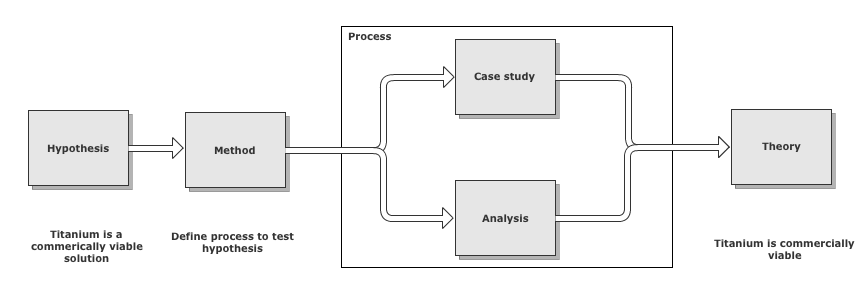
\includegraphics[scale=0.5]{images/process.png}\\{Main research process schematic}\\
\end{centering}

% summarize + go ahead for the next two chapters.
%\paragraaf{Summary}
%To answer whether or not the chosen solution is commercially viable a case study will be performed during which the solution will be analyzed on provided criteria.


\hoofdstuk{Titanium analysis}

\paragraaf{Introduction}
Work in progress
%korte herhaling van wat titanium is, referentie naar existing solutions.
This chapter will analyze how Titanium works and why it provides the desired native \emph{look-and-feel}.
flexibility, extensibility

In this chapter we will attempt to analyze 

\paragraaf{Inner workings}

At runtime a mobile application developed with Titanium consists of three major components:
\begin{itemize}
	\item
	The JavaScript source code
	\item
	A platform-specific implementation of the Titanium API
	\item
	A JavaScript interpreter
\end{itemize}

During runtime the JavaScript source code will be integrated in a native class where it is encoded as a string and compiled. The implementation of the Titanium API done in a platform specific native programming language, Java for Android and Objective-C for iOS. The JavaScript interpreter evaluates the JavaScript code at runtime.


\subparagraaf{Runtime}
At runtime a JavaScript execution environment set up in the native environment, this is where the application source code is evaluated. Injected into JavaScript execution environment are so called \emph{proxy} objects.

\subparagraaf{Proxy objects}
A proxy object is an JavaScript object paired to an object in native code.\cite{Whinnery2012} This means the object exists in both JavaScript and native code. Proxy objects gap the bridge between the native and the JavaScript environment. A global Titanium object in JavaScript exposes access to the proxy objects. 

% So, for example var label = Titanium.UI.createTabel({ text: "label" }); will invoke a native method which creates a native UILabel object. 

% var b = Ti.UI.createButton({title:'Title'});, that will invoke a native method that will create a native UI object, and create a “proxy” object (b) which exposes properties and methods on the underlying native UI object to JavaScript.
% UI components (view proxies) can be arranged hierarchically to create complex user interfaces. Proxy objects which represent an interface to non-visual APIs (like filesystem I/O or database access) execute in native code, and synchronously (or asynchronously for APIs like network access) return a result to JavaScript. 


For example: In the JavaScript code, when a function is called on the global Titanium object to create a native UILabel a proxy object is created.
\   : voorbeeld afmaken
\begin{minted}[mathescape,
			   label="JavaScript-object",
               linenos,
               numbersep=5pt,
               gobble=0,
               frame=lines,
               framesep=2mm]{js}

var label = Titanium.UI.createTabel({
   text: "Lorem impsum",
   top: 10,
   left: 10,
   width: 100,
   height: 20
});
\end{minted}


In iOS the proxy button object:

\begin{minted}[linenos,
				label="Native-object",
				samepage,
				tabsize=2,
				xleftmargin=0cm,
               numbersep=5pt,
               frame=lines,
               framesep=2mm]{objc}
-(UILabel*)label
{
    if (label==nil)
    {
        label = [[UILabel alloc] initWithFrame:CGRectZero];
        label.backgroundColor = [UIColor clearColor];
        label.numberOfLines = 0;
        [self addSubview:label];
    }
    return label;
}
\end{minted}

\subparagraaf{JavaScript}
% %TODO verwoorden:
% JavaScript (sometimes abbreviated JS) is a prototype-based scripting language that is dynamic, weakly typed and has first-class functions. It is a multi-paradigm language, supporting object-oriented,[5] imperative, and functional[1][6] programming styles.
% JavaScript was formalized in the ECMAScript language standard and is primarily used in the form of client-side JavaScript, implemented as part of a Web browser in order to give enhanced user interfaces and dynamic websites. This enables programmatic access to computational objects within a host environment.
% JavaScript's use in applications outside Web pages — for example in PDF documents, site-specific browsers, and desktop widgets — is also significant. Newer and faster JavaScript VMs and frameworks built upon them (notably Node.js) have also increased the popularity of JavaScript for server-side web applications.
% JavaScript uses syntax influenced by that of C. JavaScript copies many names and naming conventions from Java, but the two languages are otherwise unrelated and have very different semantics. The key design principles within JavaScript are taken from the Self and Scheme programming languages.[7]


As mentioned above, Titanium uses JavaScript for cross-platform code compatibility. JavaScript is a logical choice because there are JavaScript Interpreters available for most platforms. This includes the targetted mobile platforms:

V8 is the default for Android but Rhino is also supported. V8 is has a better performance dealing as Rhino because it is directly intergrated to the NDK\footnote{Native Development Kit}. This means the code does not have to run trough the JVM\footnote{Java Virtual Machine}. Performance gain can exceed over 200\% processing time when parsing a JSON object.\cite{Lukasavage2011}
For iOS JavaScriptCore is the choosen interpreter.

These interpreters support the CommonJS specification.


\subparagraaf{CommonJS}
%TODO: verwoorden:
JavaScript is a powerful object oriented language with some of the fastest dynamic language interpreters around. The official JavaScript specification defines APIs for some objects that are useful for building browser-based applications. However, the spec does not define a standard library that is useful for building a broader range of applications.

The CommonJS API will fill that gap by defining APIs that handle many common application needs, ultimately providing a standard library as rich as those of Python, Ruby and Java. The intention is that an application developer will be able to write an application using the CommonJS APIs and then run that application across different JavaScript interpreters and host environments. With CommonJS-compliant systems, you can use JavaScript to write:

Server-side JavaScript applications
Command line tools
Desktop GUI-based applications
Hybrid applications (Titanium, Adobe AIR)



\subparagraaf{Modules}
%TODO: verwoorden:
By default, JavaScript runs programs in a global scope and doesn't have any native namespacing language features. This means that, unless you're careful, your programs can descend into a mess of code spaghetti, full of conflicting variables and namespace pollution.

CommonJS modules are one of the best solutions to JavaScript dependency management.

CommonJS modules solve JavaScript scope issues by making sure each module is executed in its own namespace. Modules have to explicitly export variables they want to expose to other modules, and explicitly import other modules; in other words, there's no global namespace.

Modules prevent variables from glogging up the global namespace.


a sample module:


\begin{minted}[mathescape,
         label="eventCell.js",
               linenos,
               numbersep=5pt,
               gobble=0,
               frame=lines,
               framesep=2mm]{js}
function eventCell(Event, delegate) {
  // cell code removed
  return this.cell;
};
module.exports = eventCell;
\end{minted}

Is used like:
\begin{minted}[mathescape,
         label="eventCell.js",
               linenos,
               numbersep=5pt,
               gobble=0,
               frame=lines,
               framesep=2mm]{js}
  var messageCell = require('stager/tableview/messageCell');
  tableview.appendRow(new messageCell(message, that));
\end{minted}

% gaat er te ver op in:
% \paragraaf{Eclipse}
% \paragraaf{Buildsystem}
% \paragraaf{XCode CLI and the iOS SDK}
% \paragraaf{Android SDK}

\paragraaf{Usage concepts}
\subparagraaf{Window Navigation}
\subparagraaf{View hierarchie}
\subparagraaf{Event handling}

\paragraaf{Extensibility and flexibility}
\subparagraaf{Module system}

\paragraaf{Performance versus flexibility}
tableview.

\paragraaf{Documentation}
all in one place
wide range: video tutorials to confluence based guides


\paragraaf{Summary}
% werking, architectuur, kort samenvatten
Titanium provides the \emph{native look-and-feel} trough proxy objects. 

\hoofdstuk{Case study}

\paragraaf{Introduction}
Mobile application has been developed with Titanium to study its flexibility and features.


\paragraaf{Stager}
In 2011, live music venue WORM hired Lunatech to build \emph{Stager}, a modern web-based resource planning and ticketing application to help manage live music events. Lunatech took the opportunity to use the relatively new Play framework to build a web application with an HTML5 and Java architecture. Stager has broad requirements ranging from high performance and security for the public ticket sales component to high usability for the internal resource planning component that will be used for hours a day by employees and being open to enhancements in the future for new customers. \cite{Lunatech2011}

\subparagraaf{WORM}
WORM is an institute for avantgardistic recreation Rotterdam, consisting of an artistscollective, a podium with a bar and Parallel University (DIY workshops for film, music and media). Born under the stars of punk, Dada, Fluxus, Situationism and futurism WORM is grown into a headstrong organization that the 'Do-It-Yourself' mentality of their ancestors, combined with ultra-pragmatism, love of technique (s) and proper accounting. Worm outputs film, radio, concerts, courses, partys, publications, performances, web projects, installations, workshops and an accumulation of tactile media and internet.WORM focuses (cheerful yet serious) in avantgarde, resource scarcity and opensource. \cite{WORM2012}

\paragraaf{Stager app}
As described in the chapter \emph{Background} Stager is an planning and ticketing application to help manage live music events. In addition to planning and ticketing Stager features an \emph{atomfeed} to publish events. A Stager app would make use of this atomfeed to list any published events on a mobile device.


\paragraaf{Stager application requirements}

List of current and upcoming events
events are downloaded in JSON format from the Stager event atomfeed at /web/feeds/events
events are displayed in a row-based layout
events are linked to their corresponding event detailview
events in the list are sorted by date (asc)
events in the list contain labels with event title, subtitle, date

Detailview of an event
Shows detailed event information of an selected event:
event title, 
subtitle, 
date, 
times (doors open, start, end), 
location details (venue name, street, number, city), 
event content (html rendered text)

Add event to agenda
Prompts the user: "Add event 'x' on date 'y' in agenda?"
Adds a selected event to the mobile devices agenda.
Prompts the user of succes of add action.

Start gps-based navigation towards physical location of event
Prompts the user "Navigate to y?" (y in the format of: streetname, housenumber, cityname, postalcode)
Opens map application with address as argument.

View media attached to an event
Media defined as: URL's to event images, videos, websites.

Display in a grid or list, categorize media types.
Each displayed media item is resembled by a tumbnail or icon.
When selected a media item opens to its content in:
images an included webview,
websites the device browser,
for videos the youtube app or the browser( depending on video type \& location).

Share event details to social media
An event detail view will contain a 'share/deel' button.
Prompts the user for platform to share. (twitter/facebook/email)
Default value (editable): "I am attending event x on date y in location x !"

	
(Un)Register device to receive push notifications on new events of interest
Register the device to receive pushed notifications about upcoming events which might be of interest to the user.
Based on Relation.interest model in Stager.



\subparagraaf{Events}



\subparagraaf{Notifications}
\subparagraaf{Tickets}
\subparagraaf{i18n}
\subparagraaf{Mobile payment}
\paragraaf{Used techniques and methodologies}
\subparagraaf{Javascript}
For Titanium Javascript is the only option. Everything that can be written in JavaScript will eventually be written in JavaScript.
\subparagraaf{CommonJS}
\subparagraaf{Playframework}
\subparagraaf{Java}
\subparagraaf{JSON}
%\paragraaf{Titanium modules}
%\paragraaf{Stager service modules}


\paragraaf{Conclusion}
%Samenvatten wat er gedaan is aan de Stager app, welke platforms het draaid, e.d.

\paragraaf{Results}



